\documentclass[12pt,letterpaper]{article}
\usepackage[utf8]{inputenc}
\usepackage{amsmath}
\usepackage{amsfonts}
\usepackage{amssymb}
\usepackage{amsthm}
\usepackage{graphicx}
\usepackage{tabularx}
\usepackage[left=2cm,right=2cm,top=2cm,bottom=2cm]{geometry}
\usepackage{fancyhdr}
\usepackage{multicol}
\usepackage{multirow,array}
\usepackage{newtxtext,newtxmath}
\usepackage{relsize}
\usepackage{lastpage}
\usepackage{cancel}
\usepackage{tikz}
\usepackage{enumitem}
\usepackage{adjustbox}
\newcolumntype{Y}{>{\centering\arraybackslash}X}
\setenumerate[1]{label={\bf \theenumi: ~}}
\setenumerate[2]{label={\bf \theenumii: ~}}
\pagestyle{fancy}
\fancyhf{}
\lhead{\textsc{BHCC Mat-181}}
\rhead{\textsc{One-sample Hypothesis Tests}}
\rfoot{Page \thepage ~of \pageref{LastPage}}

\newcommand*\circled[1]{\tikz[baseline=(char.base)]{
            \node[shape=circle,draw,inner sep=2pt] (char) {#1};}}
\newcommand{\N}[2]{\mathcal{N}\big(#1,~#2\big)}
\newcommand{\Geo}[1]{\texttt{Geo}\big(#1\big)}
\newcommand{\B}[2]{\mathcal{B}\big(#1,~#2\big)}

\begin{document}
\begin{enumerate}

\item A fair 6-sided die should have a population mean $\mu=3.5$ and a population standard deviation $\sigma=1.708$. To check the fairness of a die, you are asked to perform a sampling of size $n=100$ and two-tailed hypothesis test with significance level $\alpha = 0.05$. 
\begin{enumerate}
\item State the hypotheses.
\vfill
\item Describe and sketch the null's population distribution. Use $X_0$ as the random variable.
\vfill
\item Describe and sketch the null's sampling distribution (with $n=100$). Let $\overline{X_0}$ be the random variable.
\vfill
\item Determine $r$ such that $P\Big(\big|\,\overline{X_0}-3.5\big| \ge r \Big) = \alpha$. Then describe what $r$ means in context.
\vfill
\item Your sample yielded $\bar{x} = 3.3$. Determine the test statistic ($z$) and $p$-value. Also, make a conclusion. In this case, $p\text{-value} = P\Big(\big|\,\overline{X_0}-3.5\big| \ge 0.2 \Big) $.
\vfill
\end{enumerate}

\newpage


\item Someone guessing on a 4-choice question has a 25\% chance of success (worth 1 point) and a 75\% chance of failure (worth 0 points). This means $\mu = 0.25$ and $\sigma = \sqrt{(0.25)(0.75)} = 0.433$ (Bernoulli distribution). 

You wonder whether Jules will randomly guess on all 36 questions on a test. You decide to use a one-tailed test with $\alpha=0.05$ to decide whether Jules is doing better than random guessing.

\begin{enumerate}
\item State the hypotheses.
\vfill
\item Describe and sketch the null's population distribution (the probability distribution of a single random guess). Use $X_0$ as the random variable.
\vfill
\item Describe and sketch the null's sampling distribution (with $n=36$). Let $\overline{X_0}$ be the random variable.
\vfill
\item Determine $c$ such that $P\Big(\overline{X_0} \ge c \Big) = \alpha$. Then describe what $c$ means in context.
\vfill
\item Your sample yielded $\bar{x} = 0.389$ (because Jules got 14 questions right). Determine the test statistic ($z$) and $p$-value. Also, make a conclusion. In this case, $p\text{-value} = P\Big( \overline{X_0} \ge 0.389 \Big) $.
\vfill
\end{enumerate}

\newpage


\item Harold read that he has a 20\% chance to win a scratch-off lottery each time he plays. Thus, on average he should only have to wait $\mu=5$ times before winning, with a standard deviation of $\frac{\sqrt{1-0.2}}{0.2}=4.47$ (geometric distribution). Harold wants to run a two-tail hypothesis test with a significance $\alpha=0.02$ on the mean waiting time until success. 

For the next 60 successes, Harold tracks how many tickets it takes until success. 

\begin{enumerate}
\item State the hypotheses.
\vfill
\item Describe and sketch the null's population distribution. Use $X$ as the random variable.
\vfill
\item Describe and sketch the null's sampling distribution (with $n=60$). Let $\bar{X}$ be the random variable.
\vfill
\item Determine $r$ such that $P\Big(\big|\bar{X}-\mu_0\big| \ge r \Big) = \alpha$, where $\mu_0$ is the null's mean. Then describe what $r$ means in context.
\vfill
\item Herold's sample yielded $\bar{x} = 5.6$ . Determine the test statistic ($z$) and $p$-value. Also, make a conclusion.
\vfill
\end{enumerate}







\newpage


\item A company claims the average weight of a trinket is 100 pounds. You decide to test their claim with a random sample and two-tail hypothesis test with a significance level of 0.05.
\begin{enumerate}
\item Describe the hypotheses.
\vfill
\item You measure 40 trinkets, yielding a sample mean of 98.8 pounds with a standard deviation of 10 pounds. Using $\sigma \approx 10$, describe the sampling distribution {\bf under the null hypothesis}. (Give the type of distribution and its parameters.)
\vfill
\item Determine the test statistic ($z$) of the observation. In other words, determine a $z$ score of the observed sample mean in the null's sampling distribution.
\vfill
\item Determine a $p$-value. Also make a conclusion.
\vfill
\end{enumerate}

\newpage

\item You wonder if $\mu$ is 888. You decide to do a 2-tail hypothesis test with a significance level of 0.05. A random sample of size 50 is taken, yielding $\bar{x} = 851$ and $s=106$. 
\begin{enumerate}
\item Describe the hypotheses.
\vfill
\item Describe the null's sampling distribution by assuming $\sigma \approx s$.
\vfill
\item Describe the $p$-value using a probability expression.
\vfill
\item Find the test statistic and $p$-value.
\vfill
\item Make a final judgement.
\vfill
\end{enumerate}

%\newpage

%\item A friend suggests that $\mu=4$ and $\sigma=5$. You take a sample ($n=30$) and find $\bar{x} = 1.9$. Do you believe your friend? Why?


\newpage

\item When a fair coin is flipped, it lands tails 50\% of the time. Kimberly has a coin, and she wonders if it is fair. She plans to flip the coin 100 times, record the proportion of tails, and perform a hypothesis test with a significance level of 0.05.
\begin{enumerate}
\item Describe the hypotheses.
\vfill
\item Determine $p$ and $\sigma$ of a single flip under the null hypothesis. (Bernoulli trial)
\vfill
\item Determine $p$ and $SE$ of the sampling distribution under the null hypothesis.
\vfill
\item Kimberly flips the coin 100 times and gets 57 tails, giving $\hat{p} = 0.57$. {\bf Determine the test statistic}, $z$, of this observation under the null's sampling distribution.
\vfill
\item Determine a $p$-value, where $p$-value $=P(|\hat{p}-p_0| > 0.07)$ assuming $H_0$ is true.
\vfill
\item What conclusion will Kimberly make?
\vfill
\end{enumerate}
\end{enumerate}

\newpage
\chead{\textsc{Answers}}
\begin{multicols}{2}
\begin{enumerate}
\item \begin{enumerate}
\item $H_0: ~~ \mu = 3.5$\\ 
$H_0: ~~ \mu \ne 3.5$
\item \begin{tabular}{|c | c c c c c c |} \hline
$x_{0i}$ & 1 & 2 & 3 & 4 & 5 & 6 \\ \hline
$P(X_0 = x_{0i})$ & $\frac{1}{6}$ & $\frac{1}{6}$ & $\frac{1}{6}$ & $\frac{1}{6}$ & $\frac{1}{6}$ & $\frac{1}{6}$  \\ \hline
\end{tabular} \\
$X_0$ is uniformly distributed across its 6 discrete possibilites (1 through 6).
\\ 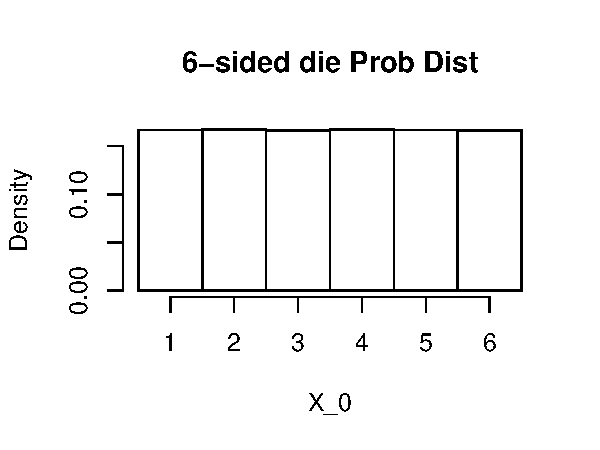
\includegraphics[scale=0.7]{code/dice_hist}
\item We calculate $SE = \frac{1.708}{\sqrt{100}} = 0.1708$, so $\overline{X_0} \sim \N{\mu=3.5}{\sigma=0.1708}$. \vspace{-15pt}
\\  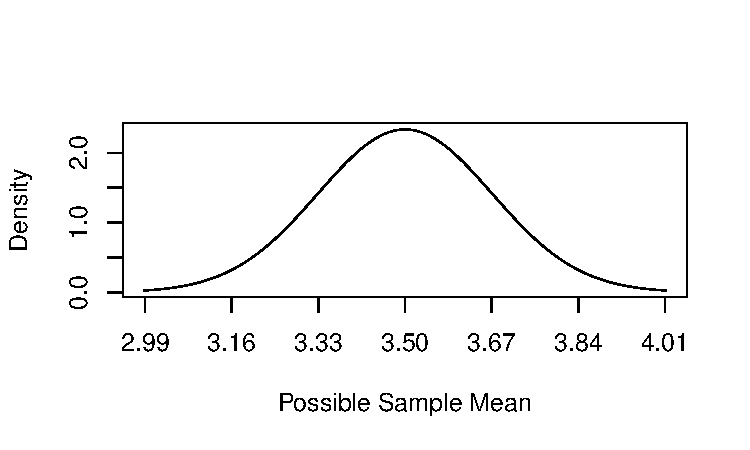
\includegraphics[scale=0.6]{code/dice_samp_hist}
\item You should sketch a picture. We recognize we need the two-tail area to equal 0.05. We determine $z_{\alpha}$ such that $P(Z<z_{\alpha}) = 0.025$. That gives $z_{\alpha}= - 1.96$. We convert this into a $\bar{x_{\alpha}}$ value. $\bar{x_{\alpha}} = 3.5 - (1.96)(0.1708)$, giving 3.17, which is 0.33 units from the mean. Thus, $r=0.33$. In this context, $r$ is how far an observed mean can be from 3.5 before we reject the null hypothesis.
\item You should sketch a picture. We want two-tail area below 3.3 and above 3.7. We find a $z$ score. $z=\frac{3.3-3.5}{0.1708} = -1.17$. We determine the left area associated with $z=-1.17$. \\$P(Z<-1.17) = 0.121$. We double this for the two-tailed area. $p$-value $=0.242$. \\
We retain the null hypothesis! This die seems fair to me.
\end{enumerate}

\item \begin{enumerate}
\item $H_0:~~ \mu=0.25 $ \\
$H_A:~~ \mu>0.25 $
\item $X_0 \sim Bernoulli(0.25)$. 
\\ 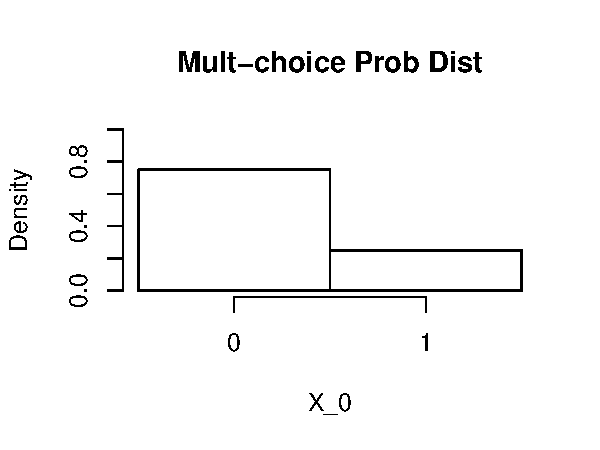
\includegraphics[scale=0.7]{code/mult_choice}
\item We calculate $SE=\frac{0.433}{\sqrt{36}} = 0.072$, leading to $\overline{X_0} \sim \N{0.25}{0.072}$.
\\ 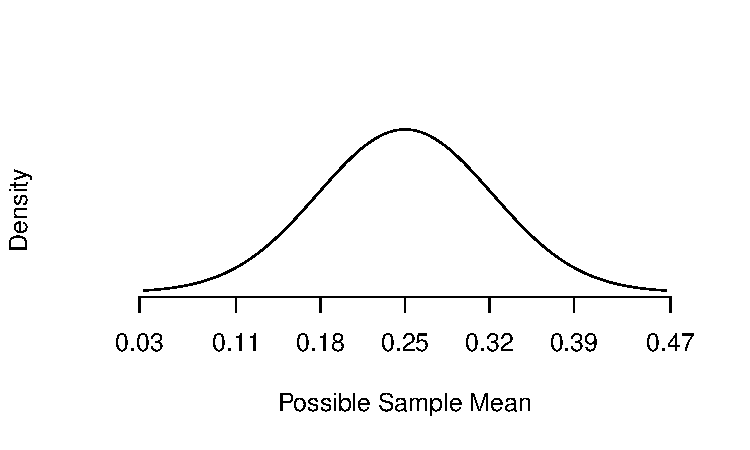
\includegraphics[scale=0.6]{code/mult_samp_hist}
\item $c=0.369$. In this context, $c$ is the cutoff mean for us deciding whether or not Jules is merely guessing.
\item $z = \frac{0.389-0.25}{0.072} = 1.93$. We use the $z$ table to find $P(Z > 1.93) = 0.0268$. So, $p$-value $=0.0268$. We reject the null hypothesis. Jules is NOT merely guessing!
\end{enumerate}

\newpage

\item \begin{enumerate}
\item $H_0:~~\mu = 5$\\
$H_A: ~~\mu \ne 5$
\item $X\sim \Geo{0.20}$.
\\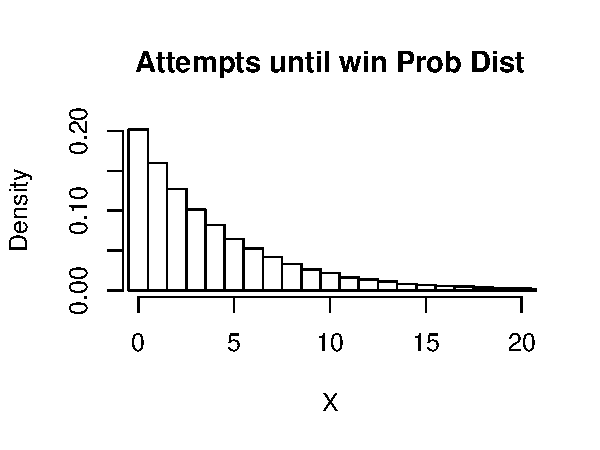
\includegraphics[scale=0.7]{code/geo_hist}
\item We calculate $SE=\frac{4.47}{\sqrt{60}} = 0.577$. So, $\bar{X} \sim \N{5}{0.577}$.
\\ 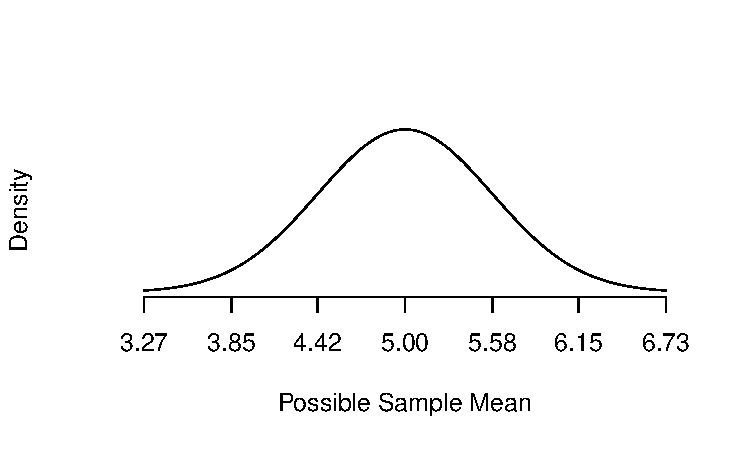
\includegraphics[scale=0.6]{code/geo_samp}
\item We find $z$ from $P(Z>z) = 0.01$, giving $z=2.32$. We can find the corresponding distance from mean, $r=z\cdot SE = 2.32 \cdot 0.577=1.34$. In this context $r$ represents a cutoff distance, between observed mean and $\mu_0$, for rejecting the null.
\item We find $z^{\star}=\frac{5.6-5}{0.577}=1.04$. We find $P(|Z| > z^{\star}) = 0.298$. We retain the null. 
\end{enumerate}


\item \begin{enumerate}
\item $H_0: ~~\mu=100$\\
$H_A: ~~\mu \ne 100$
\item The sampling distribution is normal. We calculate standard error,\\ $SE = \frac{10}{\sqrt{40}} = 1.58$. \\So, $\bar{X}\sim \N{100}{1.58}$.
\item $z = \frac{98.8-100}{1.58} = -0.759$. 
\item For this two-tailed test, we determine $P(|Z| > 0.759) = 0.447$. We retain the null hypothesis.
\end{enumerate}

\columnbreak

\item \begin{enumerate}
\item $H_0: ~~\mu=888$\\
$H_A: ~~\mu \ne 888$
\item We find $SE=\frac{106}{\sqrt{50}} = 15$.\\ So, $\bar{X}\sim\N{888}{15}$.
\item Let $\bar{X}$ represent a random draw from the null's sampling distribution.  \\$p$-value $= P(|\bar{X}-\mu_0| > 37)$. \\I got 37 from the absolute difference between 888 and 851.
\item $z=\frac{851-888}{15}=-2.47$. \\$P(|Z|>2.47) = 0.0136$.\\
$p$-value is 0.0136.
\item We reject the null hypothesis. 
\end{enumerate}

\item \begin{enumerate}
\item $H_0: ~~p=0.5$\\
$H_A: ~~p\ne 0.5 $
\item Under the null, $p=0.5$ and (Bernoulli) $\sigma = \sqrt{(0.5)(0.5)} = 0.5$. This population distribution is a Bernoulli distribution.
\item The sampling distribution is normal, with the same proportion as the population. $p=0.5$. However, the SE is smaller than $\sigma$. \\
$SE = \frac{\sigma}{\sqrt{n}} = \frac{0.5}{\sqrt{100}} = 0.05$
\item $z = \frac{\hat{p}-p_0}{SE} = \frac{0.57-0.5}{0.05} = \fbox{1.4}$.
\item We find $P(|Z|>1.4) = 0.1615$.
\item Kimberly retains the null hypothesis. For now she is still satisfied that the coin seems fair.
\end{enumerate}

\end{enumerate}
\end{multicols}
\end{document}

